\documentclass[../main.tex]{subfiles}
\graphicspath{{\subfix{../images/}}}

\begin{document}

\chapter{Results}
Fig. \ref{fig:performancetraining} shows the performance trends for the four training tasks (\textit{Path, Rings, Pillars} and \textit{Exchange}), where the performance at each repetition is the average among the subjects in the assisted or control group. Apart from the \textit{Pillars} task, the trends are increasing both for the assisted group and the unassisted group. Most significantly, the performance in the assisted group is consistently higher than the one in the control group in all training tasks. 

\begin{figure}[h!]
    \centering
    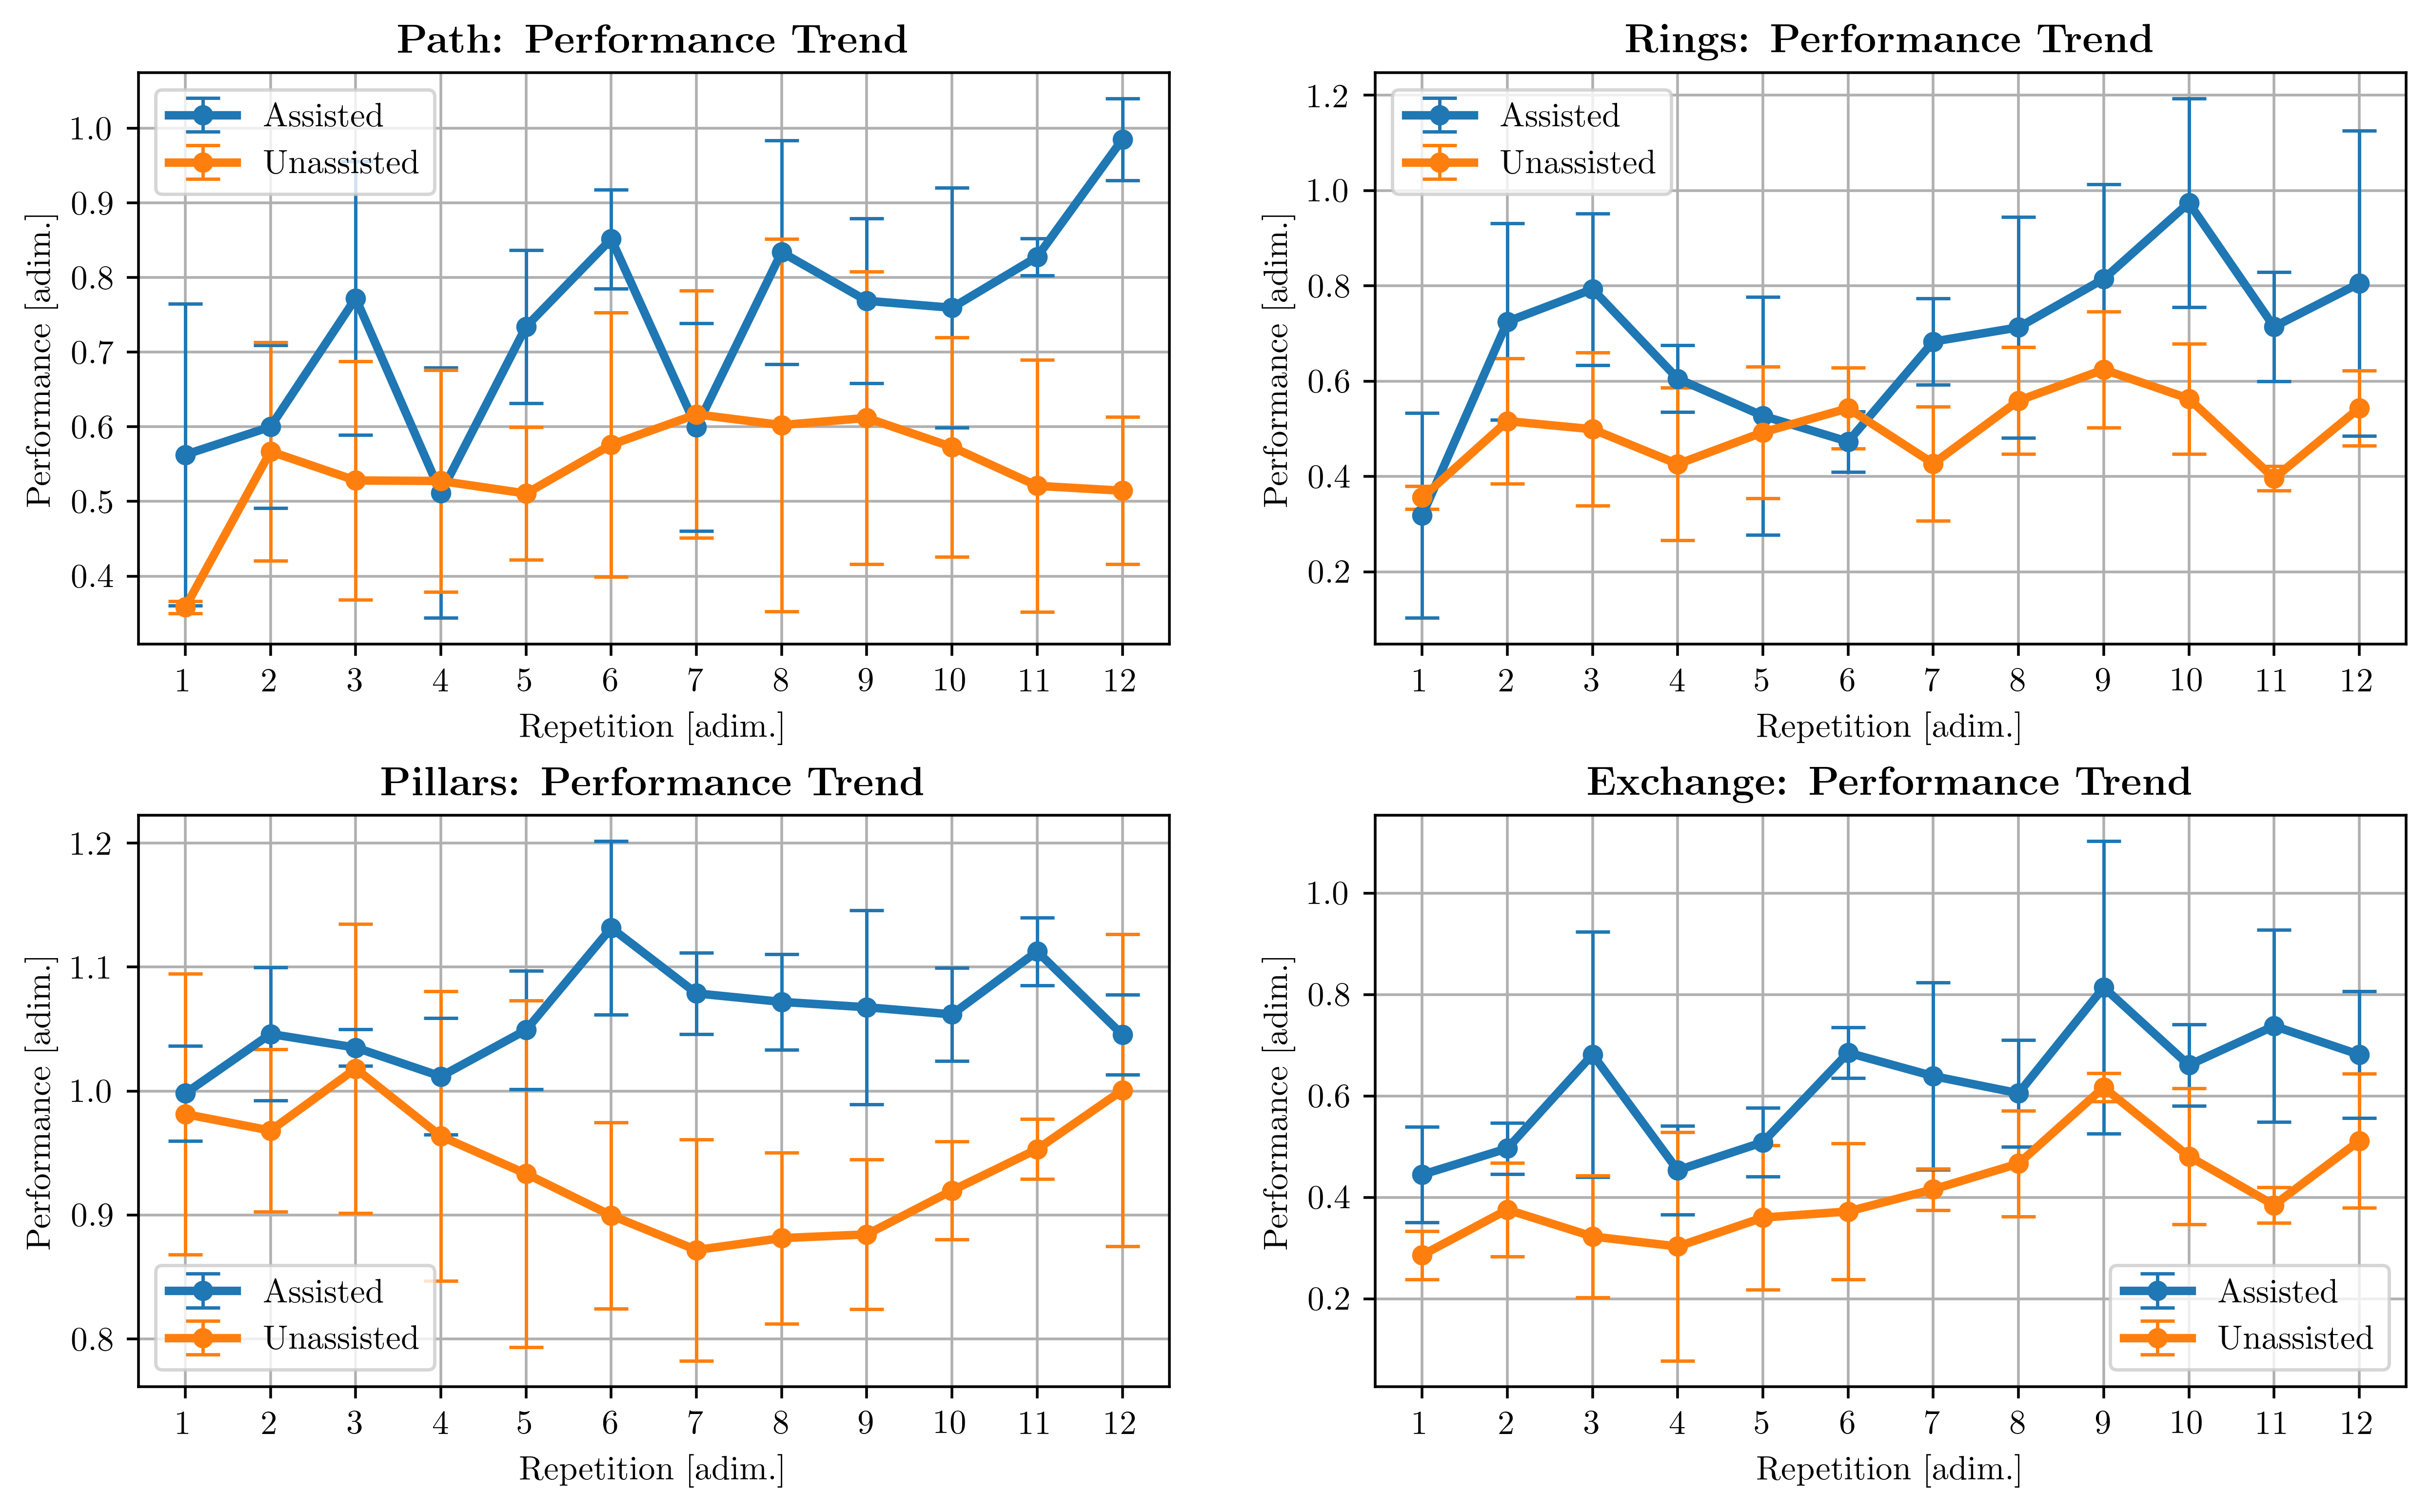
\includegraphics[width=\textwidth]{images/performance_training.png}
    \caption{Performance Trend for the four Training Tasks. The value at each repetition is averaged across the subjects belonging to the same group. Error bars show the standard variation at each repetition}
    \label{fig:performancetraining}
\end{figure}

The standard deviation of the performance score is also displayed at each repetition with error bars that denote the range $\left[\mu - \frac{1}{2}\sigma; \mu + \frac{1}{2}\sigma\right]$, with $\mu$ and $\sigma$ the mean and standard deviation of the performance score, respectively. No significant difference is observed between the two groups and neither it is present a recognizable trend of deviation as a function of repetitions, \textit{i.e.} the error bars do not get wider nor narrower as the repetitions increase.

The performance on the four validation tasks (\textit{Thymectomy, Nephrectomy, Liver Resection} and \textit{Suturing}) recorded on the last day of the experimental phase is shown in Fig. \ref{fig:performancevalidation} with boxplots. For each task, the graph reports the distribution of performances collected from the 4 subjects executing 3 repetitions. Crucially, neither the subjects in the assisted group nor the ones in the control group were guided with \acp{vf} on these tasks, nevertheless the performance recorded from the assisted subjects is distributed on higher values for all the tasks. 

\begin{figure}
    \centering
    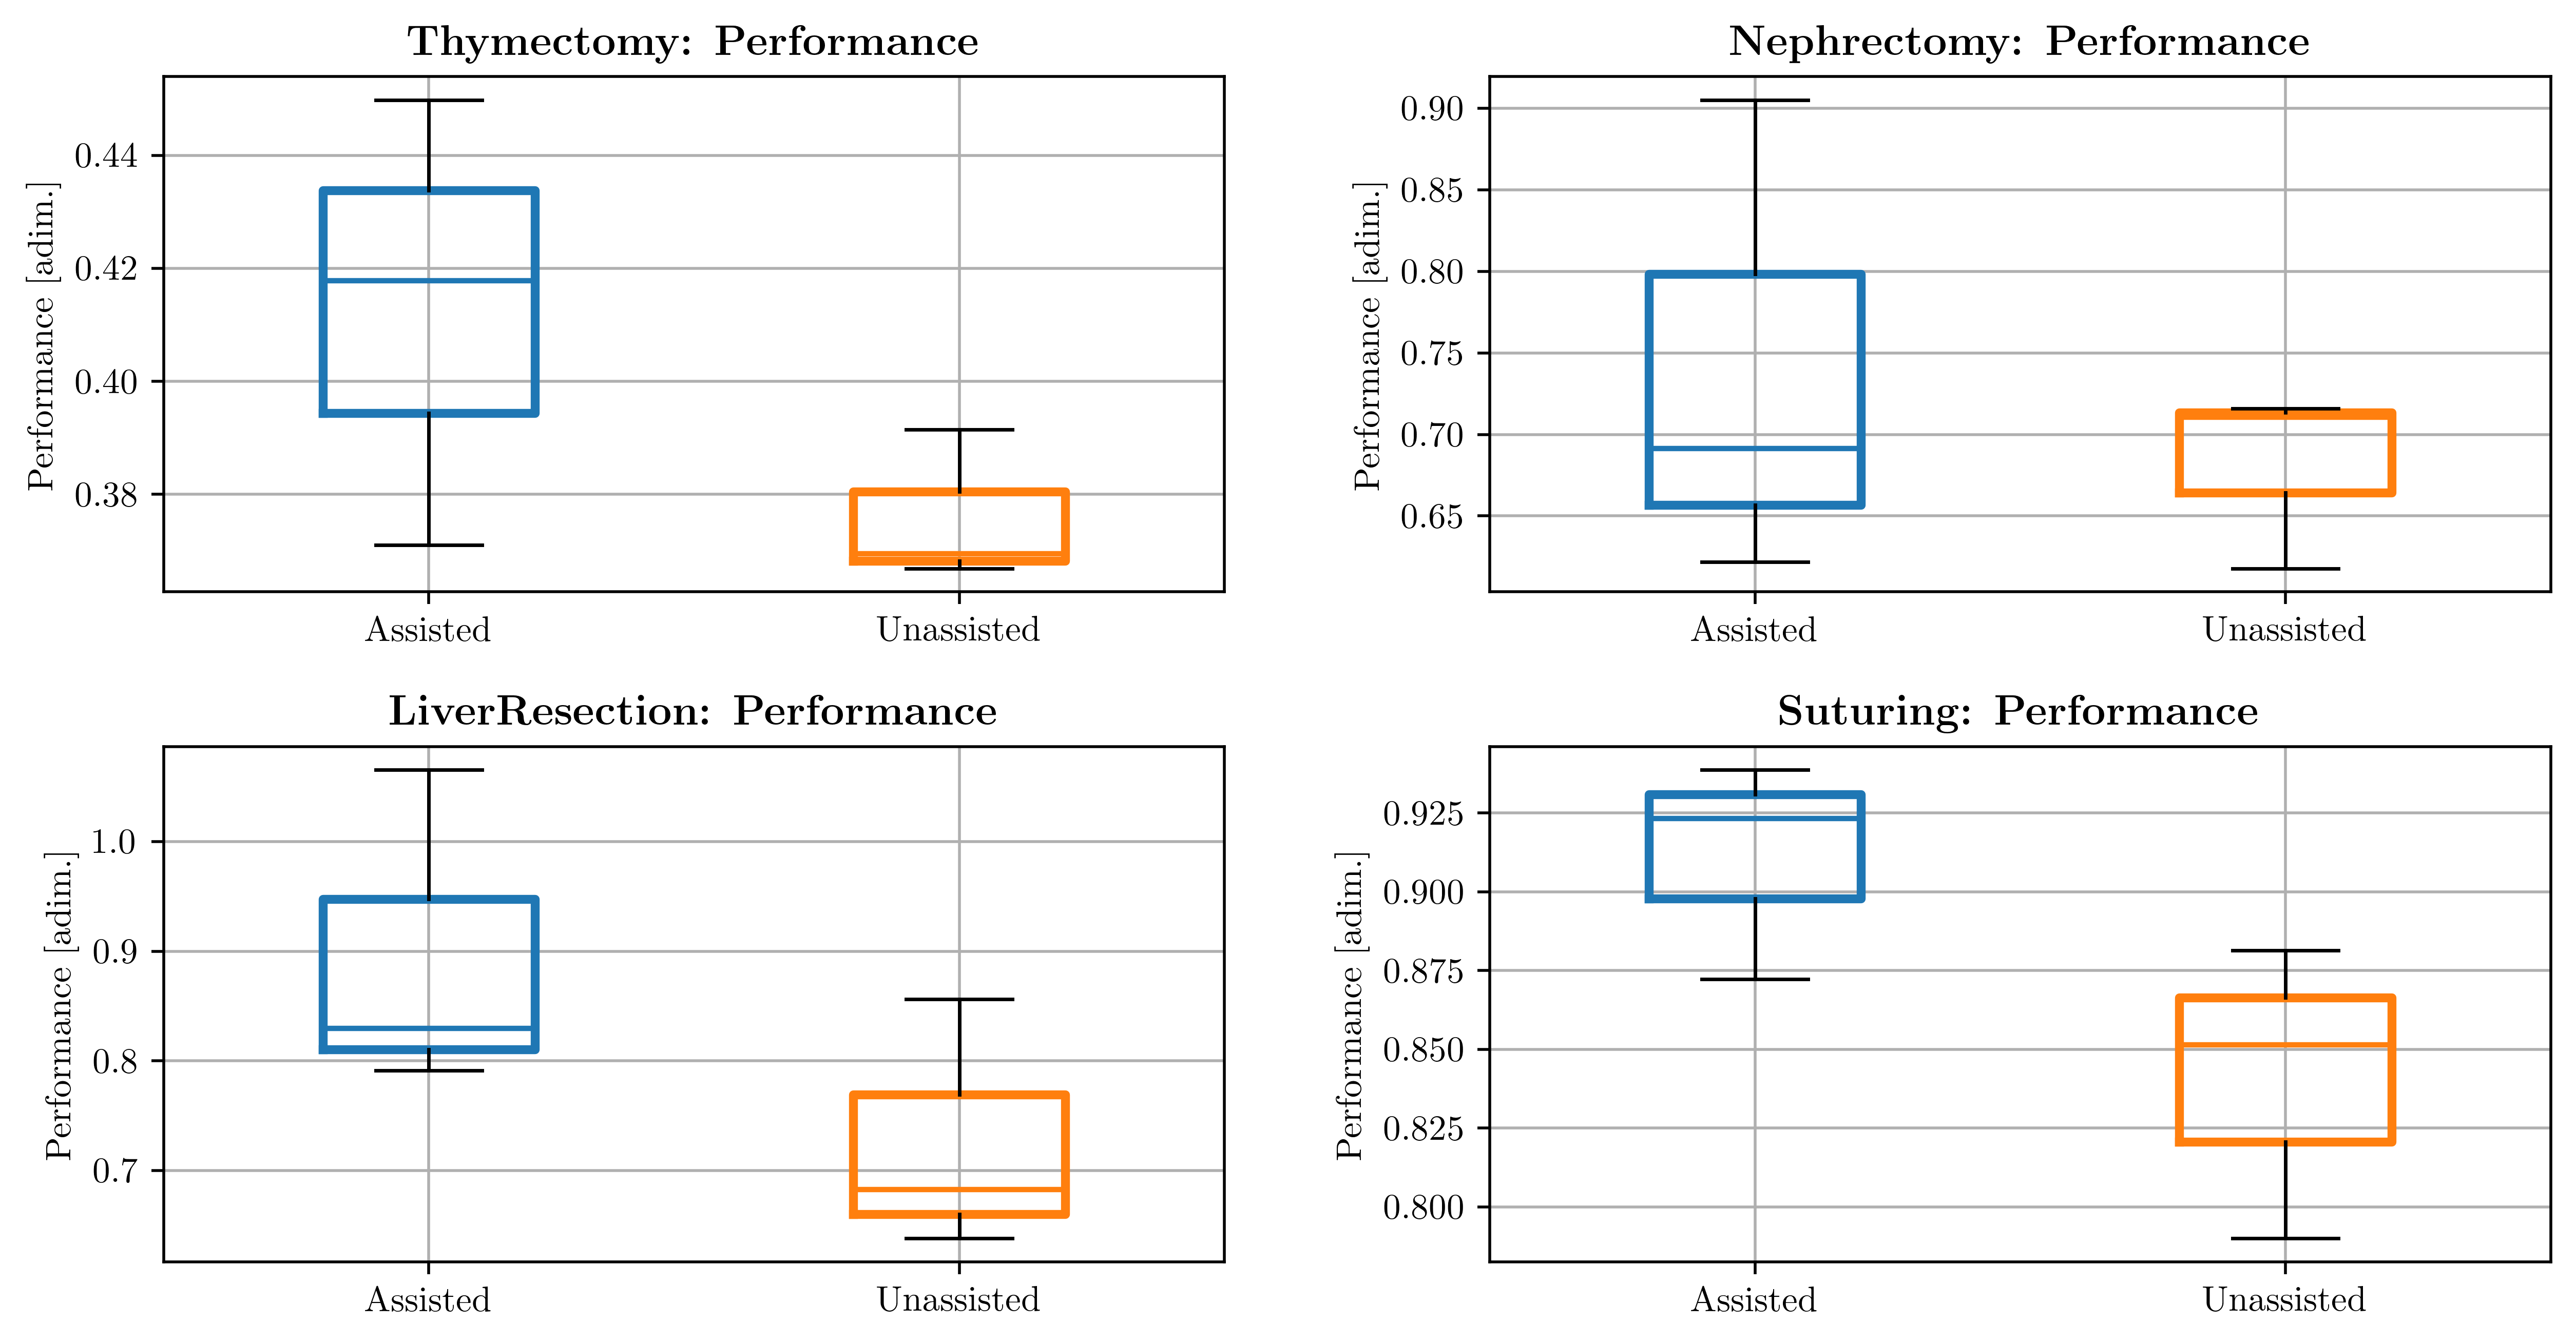
\includegraphics[width=\textwidth]{images/performance_validation.png}
    \caption{Boxplots of the average performance of assisted subjects (blue) and unassisted subjects (orange) on the four validation tasks}
    \label{fig:performancevalidation}
\end{figure}

Quantitative results are reported in the tables below: for each task, the mean, standard deviation and median values of performance are compared between the assisted and the control group. Given the data scarcity and their non-Gaussian distribution, the most meaningful conclusions will be drawn from the median values. Apart from \textit{Nephrectomy} showing a slightly reduced median performance on assisted subject (accompanied, however, by a much larger standard deviation, as per Fig. \ref{fig:performancevalidation}), all other tasks present an increase in both the mean and median performance, as high as $+21.54\%$.

The standard deviation in the performance isn't consistent when comparing the assisted and control group. 

\begin{center}
\begin{tabularx}{\linewidth}{||A|B|B|B||}
\hline
\multicolumn{4}{||c||}{\textbf{Thymectomy}} \\
\hline\hline
& Mean & STD & Median \\
\hline
CONTROL & 0.38 & 0.01 & 0.37 \\
\hline
ASSISTED & 0.41 & 0.04 & 0.42 \\
\hline
\textbf{\% VAR} & \textbf{9.83\%} & \textbf{193.94\%} & \textbf{13.07\%} \\
\hline
% \label{tab:performance_Thymectomy}
\end{tabularx}
\end{center}
\begin{center}
\begin{tabularx}{\linewidth}{||A|B|B|B||}
\hline
\multicolumn{4}{||c||}{\textbf{Nephrectomy}} \\
\hline\hline
& Mean & STD & Median \\
\hline
CONTROL & 0.68 & 0.06 & 0.71 \\
\hline
ASSISTED & 0.74 & 0.15 & 0.69 \\
\hline
\textbf{\% VAR} & \textbf{8.50\%} & \textbf{167.46\%} & \textbf{-2.71\%} \\
\hline
% \label{tab:performance_Nephrectomy}
\end{tabularx}
\end{center}
\begin{center}
\begin{tabularx}{\linewidth}{||A|B|B|B||}
\hline
\multicolumn{4}{||c||}{\textbf{LiverResection}} \\
\hline\hline
& Mean & STD & Median \\
\hline
CONTROL & 0.73 & 0.12 & 0.68 \\
\hline
ASSISTED & 0.90 & 0.15 & 0.83 \\
\hline
\textbf{\% VAR} & \textbf{23.42\%} & \textbf{28.85\%} & \textbf{21.54\%} \\
\hline
% \label{tab:performance_LiverResection}
\end{tabularx}
\end{center}
\begin{center}
\begin{tabularx}{\linewidth}{||A|B|B|B||}
\hline
\multicolumn{4}{||c||}{\textbf{Suturing}} \\
\hline\hline
& Mean & STD & Median \\
\hline
CONTROL & 0.84 & 0.05 & 0.85 \\
\hline
ASSISTED & 0.91 & 0.03 & 0.92 \\
\hline
\textbf{\% VAR} & \textbf{8.38\%} & \textbf{-25.39\%} & \textbf{8.44\%} \\
\hline
% \label{tab:performance_Suturing}
\end{tabularx}
\end{center}


% BIBLIOGRAPHY
% \bibliographystyle{unsrt}
% \bibliography{refs.bib}

\end{document}